\section{Clove}
\label{sec:clove}

\begin{spice}\label{spice:clove}
\textsc{Clove} \hfill \href{https://powo.science.kew.org/taxon/601421-1}{POWO} \\
\textbf{English:} \textit{clove}. 
\textbf{Arabic:} {\arabicfont{قرنفل}} \textit{qaranful}. 
\textbf{Chinese:} {\tc{丁香}} \textit{dīngxiāng} [nail-spice]. 
\textbf{Hungarian:} \textit{szegfűszeg} [nail-grass-nail].  \\
\noindent{\color{black}\rule[0.5ex]{\linewidth}{.5pt}}
\begin{tabular}{@{}p{0.25\linewidth}@{}p{0.75\linewidth}@{}}
Plant species: & \taxonn{Syzygium aromaticum}{(L.) Merr. \& L.M.Perry} (syn. \taxonn{Eugenia aromatica}{(L.) Baill.}); \textit{\taxonn{Eugenia cayophyllata}{Thunb.}} \\
Family: & \textit{Myrtaceae} \\
part used: & flower buds \\
Region of origin: & Moluccas (Indonesia) \\
Cultivated in: & Indonesia; Malaysia; Tanzania \\
Color: & rich, reddish brown \\
\end{tabular}
\end{spice}

\begin{figure}[!ht]
	\vspace{-4ex}
	\centering
	\subfloat[\centering a]{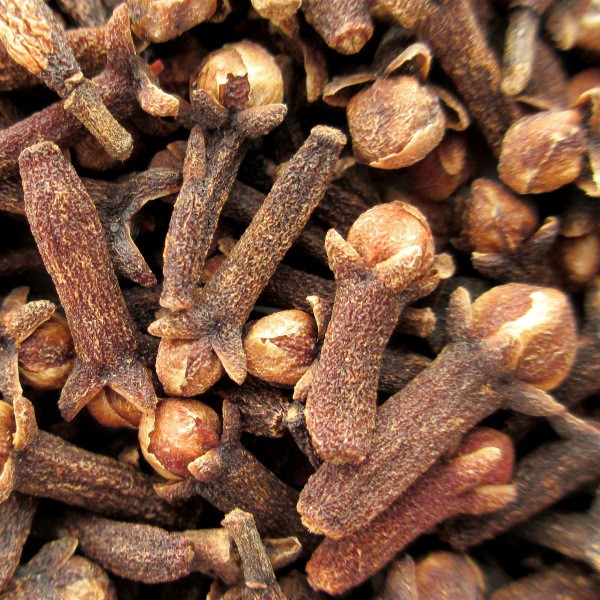
\includegraphics[width=0.3\linewidth]{imgs/spices/cloves-1.jpg}}
	\hfill
	\subfloat[\centering b]{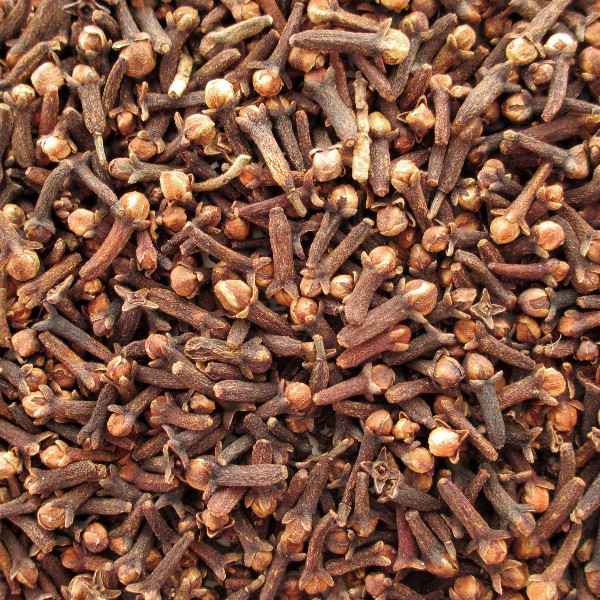
\includegraphics[width=0.3\linewidth]{imgs/spices/cloves-2.jpg}}
	\hfill
	\subfloat[\centering c]{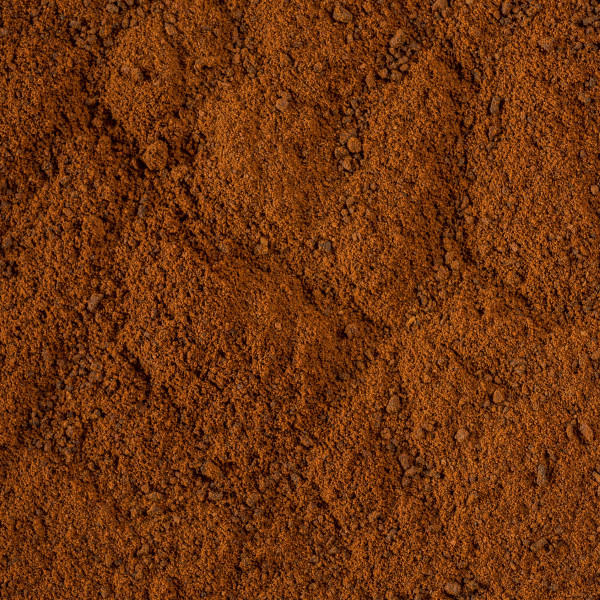
\includegraphics[width=0.3\linewidth]{imgs/spices/cloves-3.jpg}}
	\caption{Clove \textit{}.}
	\label{fig:clove_imgs}
\end{figure}

\subsection{The Botany, Origins, and Cultivation of Clove}

\subsection{The History of Clove}

\subsection{The Names of Clove}

\subsubsection{English}

\begin{etymology}\label{ety:clove}
English \textit{clove}, ?ca. 1225
< Anglo-Norman \textit{clow}, c.1200
< Old French \textit{clou}, XII
< Latin \textit{clāvus} `nail'\footnote{; }
\end{etymology}

\begin{table}[!ht]
\centering
\begin{tabularx}{\textwidth}{@{}l>{\itshape \small}lL>{\small}l@{}}
\toprule
\textbf{\#} & \multicolumn{1}{l}{\textbf{Species}} & \multicolumn{1}{l}{\textbf{Name}} & \multicolumn{1}{l}{\textbf{Source}} \\
\midrule
\textbf{1}	& \textbf{Syzygium aromaticum}	& \textbf{clove}	& \textbf{\textcite{van_wyk_culinary_2014}} \\
\bottomrule
\end{tabularx}
\caption{Various names for clove in English.}
\label{table:names_clove_en}
\end{table}



\subsubsection{Arabic}

\begin{table}[!ht]
    \caption{Various names for clove in Arabic.}
\centering
\begin{tabularx}{\textwidth}{@{}l>{\itshape \small}lr>{\itshape}lL>{\small}l@{}}
\toprule
\textbf{\#} & \multicolumn{1}{l}{\textbf{Species}} & \multicolumn{1}{l}{\textbf{Name}} & \multicolumn{1}{l}{\textbf{Tr.}} & \multicolumn{1}{l}{\textbf{Gloss}} & \multicolumn{1}{l}{\textbf{Source}} \\
\midrule
1	& Syzygium aromaticum	& كيش قرنفل	& kabsh qaranful	& ram of cloves?	& \textcite{baalbaki_-mawrid_1995} \\
\textbf{2}	& \textbf{Syzygium aromaticum}	& \textbf{قرنفل}	& \textbf{qaranful}	& \textbf{}	& \textbf{\textcite{amar_arabian_2017}} \\
\bottomrule
\end{tabularx}
\label{table:names_clove_ar}
\end{table}



\subsubsection{Chinese}

\begin{table}[!ht]
\centering
\begin{tabularx}{\textwidth}{@{}l>{\itshape \small}ll>{\itshape}lL>{\small}l@{}}
\toprule
\textbf{\#} & \multicolumn{1}{l}{\textbf{Species}} & \multicolumn{1}{l}{\textbf{Name}} & \multicolumn{1}{l}{\textbf{Tr.}} & \multicolumn{1}{l}{\textbf{Gloss}} & \multicolumn{1}{l}{\textbf{Source}} \\
\midrule
\textbf{1}	& \textbf{Syzygium aromaticum}	& \textbf{\tradchinesefont{丁香}}	& \textbf{dīngxiāng}	& \textbf{nail-spice}	& \textbf{\textcite{kleeman_oxford_2010}} \\
2	& Syzygium aromaticum	& \tradchinesefont{雞舌香}	& jīshéxiāng 	& chicken-tongue-spice	& \textcite{defrancis_abc_2003} \\
\bottomrule
\end{tabularx}
\caption{Various names for clove in Chinese.}
\label{table:names_clove_zh}
\end{table}



\subsubsection{Summary}

\begin{table}[!ht]
\centering
\begin{tabularx}{\textwidth}{@{}ll>{\itshape}lLl>{\small}l@{}}
\toprule
\textbf{\#} & \textbf{Language} & \multicolumn{1}{l}{\textbf{Term}} & \textbf{Gloss} & \textbf{Loan} & \multicolumn{1}{l}{\textbf{Source}} \\
\midrule
1	& English	& clove	& 	& yes	& \textcite{oed} \\
\midrule
1	& Arabic	& kabsh qaranful	& handful of cloves?	& 	& \textcite{baalbaki_-mawrid_1995} \\
2	& Arabic	& qaranful	& 	& yes	& \textcite{wehr_dictionary_1976} \\
\midrule
1	& Chinese	& dīngxiāng	& nail-spice	& no	& \textcite{kleeman_oxford_2010} \\
2	& Chinese	& jīshéxiāng 	& chicken-tongue-spice	& no	& \textcite{defrancis_abc_2003} \\
\bottomrule
\end{tabularx}
\caption{Conventionalized names for clove in English, Arabic, and Chinese, found in dictionaries.}
\label{table:names_clove}
\end{table}












% EE:
% dried flower-bud of tropical myrtle. XIV. orig. clow (of) gilofer — (O)F. clou de girofle (gilofre) ‘nail of clove-tree’, so called from its shape; see GILLYFLOWER. The change from clow to clove is difficult to account for.

% Wo:
% You might have two different types of clove in your kitchen cupboard, one in a jar on the spice rack and one in a garlic bulb. These are two different words. The older, the spice clove, comes from Old French clou de girofle (source of the name gillyflower [LME] for the similarly scented pink), meaning ‘nail of the clove tree’. You can see why—cloves look like nails. The clove of garlic is an Old English word related to cleave [OE] and cloven [ME].

% OEymonline:
% dried flowerbud of a certain tropical tree, used as a spice, late 15c., earlier clowes (14c.), from Anglo-French clowes de gilofre (c. 1200), Old French clou de girofle "nail of gillyflower," so called from its shape, from Latin clavus "a nail" (from PIE root *klau- "hook"). For second element, see gillyflower. The two cloves were much confused in Middle English. The clove pink is so called from the scent of the flowers.

% MW:
% alteration (probably influenced by 1clove) of Middle English clowe, cloue, from Old French clou (de girofle), literally, nail of clove, from Latin clavus nail
% First Known Use: 13th century (sense 1a)

% AH:
% [Middle English, from Old French clou (de girofle), nail (of the clove tree), from Latin clāvus, nail.]

% Wiktionary:
% From Middle English clove, an alteration of earlier clowe, borrowed from the first component of Old French clou (de girofle) (modern French clou de girofle), from Latin clāvus (“nail”) for its shape. Also see clāva (“knotty branch, club”). Doublet of clou. 

\begin{etymology}
English gillyflower (1550s),
< Middle English gilofre `gillyflower' (XIV), originally `clove' (c. 1300)
< Old French girofle, gilofre `clove' (XII)
< Late Latin caryophyllon
< Ancient Greek karyophyllon `clove, nut leaf, dried flower bud of clove tree' 
< karyon `nut' + phyllon `leaf'
\end{etymology}

% EE:
% †clove XIV; clove-scented pink, wallflower, etc. XV. ME. gilofre, gerofle — OF. gilofre, girofle — medL. caryophyllum — Gr. karuóphullon clove-tree, f. káruon nut + phúllon leaf. Alt. in Eng. (XV) by assim. to flower.

% OE: of G
% type of flowering plant, 1550s, folk etymology alteration (by association with unrelated flower) of gilofre "gillyflower" (late 14c.), originally "clove" (c. 1300), from Old French girofle "clove" (12c.), from Latin caryophyllon, from Greek karyophyllon "clove, nut leaf, dried flower bud of clove tree," from karyon "nut" (see karyo-) + phyllon "leaf" (from suffixed form of PIE root *bhel- (3) "to thrive, bloom"). The flower so named for its scent.

% MW:
% by folk etymology from Middle English gilofre, gelofer, from Middle French girofle, gilofre, from Latin caryophyllum, from Greek karyophyllon, from karyon nut + phyllon leaf — more at careen, blade
% First Known Use: 14th century (sense 1a)

% AH:
% [Alteration (influenced by FLOWER) of Middle English gilofre, from Old French gilofre, girofle, clove, from Late Latin gariofilum, from Greek karuophullon : karuon, nut; see kar- in the Appendix of Indo-European roots + phullon, leaf; see bhel-3 in the Appendix of Indo-European roots.]

% WK: of G
% By folk etymology (with influence from flower) from French girofle, gilofre, from Late Latin caryophyllum, from Ancient Greek καρυόφυλλον (karuóphullon, “dried flower buds of the clove tree”). 
